
\قسمت{الگو های طراحی}
\پاراگراف{\lr{Iterator}}

از این الگو طراحی به وفور استفاده شده است. معمولا هر جا لیست داریم، یک
\lr{Iterator}
 ای
\lr{built-in}
 که در زبان وجود دارد استفاده شده است. به صورت مثال در
\lr{UI}
در مواقع ای که کوئری ای که میگیرم جوابش به صورت لیست است، زبان
\lr{Apollo}
یک 
\lr{iterator}
 دارد که از یک عضو لیست شروع میکند و به بعدی می‌رود تا از تمام اعضای لیست دانه به دانه بگذرد. کد این
\lr{iterator}
در شکل~\رجوع{شکل:iterator-code}

\شروع{شکل}
\centering
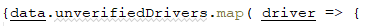
\includegraphics[width = 0.8 \linewidth]{../figs/patterns/iterator-code.png}
\برچسب{شکل:iterator-code}
\شرح{مثال \لر{Iterator} در آپولو}
\پایان{شکل}

ساختار این الگو طراحی در  شکل~\رجوع{شکل:iterator} آمده است.

\شروع{شکل}
\centering
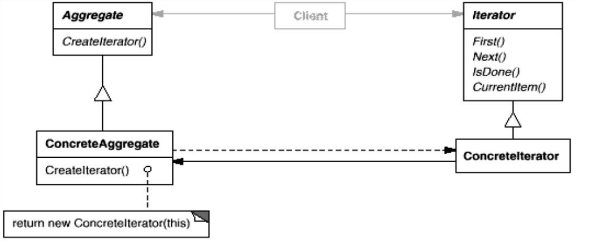
\includegraphics[width = 0.8 \linewidth]{../figs/patterns/Iterator.png}
\شرح{ساختار الگو طراحی \لر{Iterator}.}
\برچسب{شکل:iterator}
\پایان{شکل}

\پاراگراف{\lr{Singleton}}
کلاس
\lr{DriverCatalogue}
به صورت
\lr{Singleton}
است. یعنی یک تنها یک نمونه از این کلاس موجود است. در این کلاس تمام راننده ها وجود دارد. ساختار این نوع کلاس ها در شکل~\رجوع{شکل:singleton} نمایش داده شده است.

\شروع{شکل}
\centering
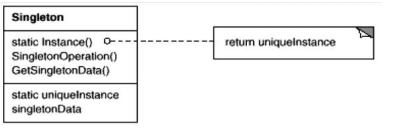
\includegraphics[width = 0.6 \linewidth]{../figs/patterns/Singleton.png}
\شرح{ساختار الگو طراحی \لر{Singleton}.}
\برچسب{شکل:singleton}
\پایان{شکل}
\پاراگراف{
\lr{Adapter}}
ما با بکاند
\lr{graphql}
کار می‌کنیم. برای همین در 
\lr{UI}
باید با استفاده از زبان 
\lr{Apollo}
 کوئری بزنیم، تا اطلاعات مورد نیاز را دریافت کنیم. اما سمت بک همیشه در حال تغییر است، و با کمی تغییر کلا کوئری های ما بهم میخورد. راهکار موجود را شرح می دهیم.

\شروع{شکل}
\centering
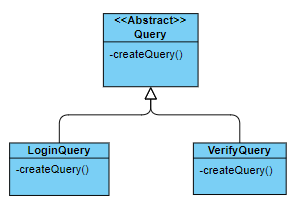
\includegraphics[width = 0.6 \linewidth]{../figs/patterns/Adapter-Adaptee.png}
\شرح{ساختار الگو طراحی \لر{Adapter}.}
\برچسب{شکل:singleton}
\پایان{شکل}
کافیست یک کلاس ابسترکت 
\lr{Query}
داشته باشیم، این کلاس یک تابع ابسترکت 
\lr{createQuery}
داشته باشد. سپس برای تولید کوئری، تابع 
\lr{createQuery}
در نمونه مورد نظر از کلاس را صدا کنیم. مثلا برای زدن کوئری 
\lr{login}
کافی است، تابع 
\lr{createQuery}
در 
\lr{LoginQuery}
صدا شود. حال اگر تغییری در کد ایجاد شد کافیست 
\lr{createQuery}
 را برابر با کوئری در کلاسی کنیم که سمت بک تعریف شده است.
